\documentclass[../ESOF_notes.tex]{subfiles}

\begin{document}
\subsection{Introduction}
\subsubsection{Software design and implementation}
\begin{itemize}
    \item It is the stage in the software engineering process at which an executable software system is developed.
    \item Its activities are invariably inter-leaved.
\end{itemize}
\subsubsection{Design levels}
\begin{itemize}
    \item \textbf{High-level design or architectural design:} partition the system into components.
    \item \textbf{Detailed design:} partition each component (or small program) into classes.
    \item Design of algorithms and data structures
\end{itemize}
\subsection{Object-oriented design using the UML}
Structured object-oriented design processes involve developing a number of different system models.
\newline
Since they require a lot of effort for development and maintenance, this models are only cost-effective for large systems.
\newline
\subsubsection{Process stages}
\begin{itemize}
    \item Define the system context and use cases;
    \item Design the system architecture;
    \item Identify the principal object classes in the system;
    \item Develop design models;
    \item Specify object interfaces (API).
\end{itemize}
\subsubsection{Design models and design views}
An object-oriented design model may in general cover 4 inter-related design views.
\begin{figure}[H]
    \centering
    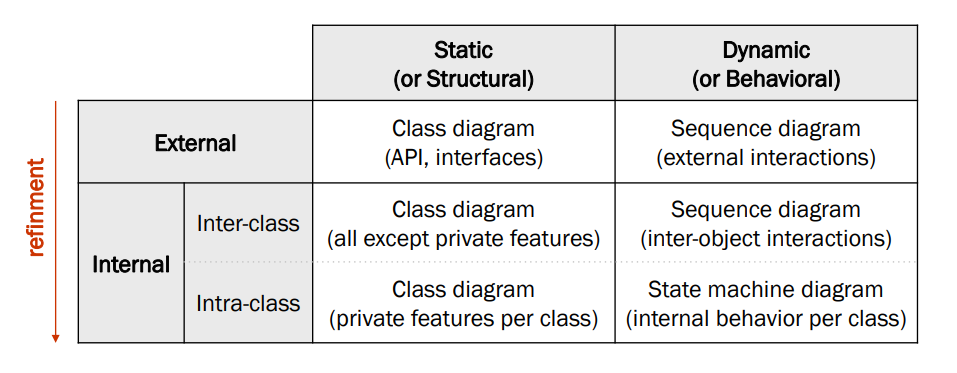
\includegraphics[scale=0.3]{design_1}
\end{figure}

\subsubsection{Sequence diagrams (SD)}
Sequence diagrams show the sequence of object interactions that take place. (usually in the context of a system use case).

\subsubsection{State machine diagrams (SMD)}
\begin{itemize}
    \item State machine diagrams are used to show how objects
          respond to different service requests and the state transitions triggered by these requests;
    \item State machine diagrams are useful high-level models of a
          system or an object’s run-time behavior;
    \item You don’t usually need a state machine diagram for all of
          the objects in the system because most objects in a system are simple.
\end{itemize}

\subsubsection{Interface specification}
\begin{itemize}
    \item Object interfaces have to be specified;
    \item Objects may have several interfaces which are viewpoints
          on the methods provide;
    \item The UML uses class diagrams for interface specification;
\end{itemize}
\subsection{Design patterns}
\begin{itemize}
    \item Way of reusing abstract knowledge about a problem and its solution;
    \item A pattern is a description of the problem and the essence
          of its solution;
    \item It should be sufficiently abstract to be reused in other cases;
    \item Pattern descriptions usually make use of object-oriented
          characteristics,
    \item Any design problem may have an associated pattern that can be applied.
\end{itemize}

\subsubsection{Pattern elements}
\begin{itemize}
    \item Name;
    \item Problem description;
    \item Solution description. (template for a design solution);
    \item Consequences (results).
\end{itemize}
\subsection{Implementation issues}
\subsubsection{Reuse}
Most modern software is constructed by reusing existing components or systems.
\newline
\newline
\textbf{Reuse levels:}
\begin{itemize}
    \item \textbf {The abstraction level:} Don’t reuse software directly but use knowledge of successful abstractions;
    \item \textbf {The object level:} Directly reuse objects from a library;
    \item \textbf {The component level:} Components are collections of objects and object classes that you reuse in application systems;
    \item \textbf {The system level:} reuse entire application systems.
\end{itemize}
\textbf{Reuse costs:}
\begin{itemize}
    \item The costs of the time spent in looking for software to reuse and assessing whether or not it meets your needs;
    \item  The costs of buying the reusable software;
    \item The costs of adapting and configuring the reusable software components or systems;
    \item The costs of integrating reusable software elements with each other and with the new code developed.
\end{itemize}
\subsubsection{Configuration management}
Configuration management is the name given to the general process of managing a changing software system.
\newline
Its aim is to support the system integration process.

\begin{figure}[H]
    \centering
    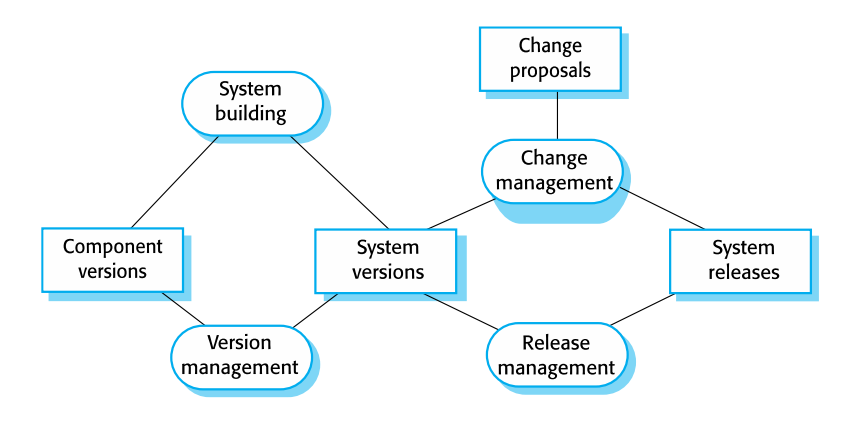
\includegraphics[scale=0.3]{design_2}
    \caption{Configuration management tool interaction}
\end{figure}

\subsubsection{Host-target development}
Most software is developed on one computer(the host), but runs on a separate machine (the target).

\begin{figure}[H]
    \centering
    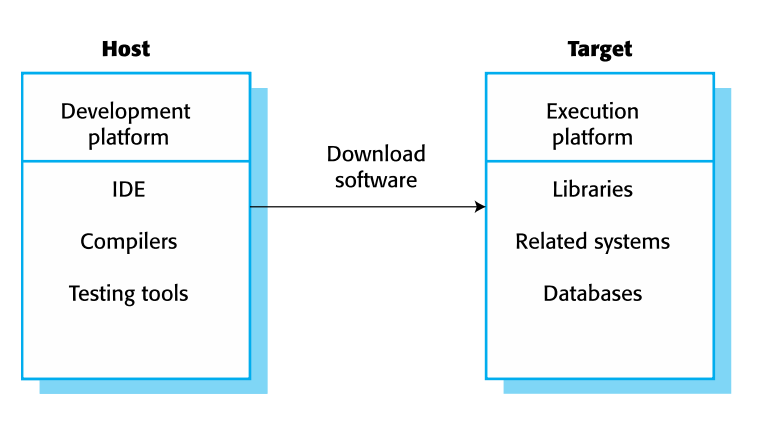
\includegraphics[scale=0.3]{design_3}
\end{figure}

\subsubsection{Development platform tools}
\begin{itemize}
    \item Integrated compiler and syntax-directed editing system that allows you to create, edit and compile code;
    \item Language debugging system;
    \item Graphical editing tools;
    \item Testing tools;
    \item Project support tools that help you organize the code for different development projects.
\end{itemize}

\subsubsection{Integrated development environments
    (IDEs)}
\begin{itemize}
    \item Software development tools are often grouped to create an integrated development environment (IDE);
    \item Is a set of tools that supports different aspects of software development;
    \item IDEs are created to support development in a specific programming language. The language IDE may be developed specially, or may be an instantiation of a general-purpose IDE.
\end{itemize}

\subsection{Key points (Design)}
Software design and implementation are inter-leaved activities. The level of detail in the design depends on the type of system and whether you are using a plan-driven or agile approach.
\newline
The process of object-oriented design includes activities to design the system architecture, identify objects in the system, describe the design using different object models and document the component interfaces.
\newline
A range of different models may be produced during an object oriented design process. These include static and dynamic models.
\newline
Component interfaces must be defined precisely so that other objects can use them.

\subsection{Key points (Implementation)}
When developing software, you should reuse existing software.
\newline
Configuration management is the process of managing changes to an evolving software system.
\newline
Most software development is host-target development. You use an IDE on a host machine to develop the software, which is transferred to a target machine for execution.
\end{document}